\section{W7-9: Gang of Four}
\begin{itemize}
    \item \textbf{Facade:} is a structural design pattern that provides a simplified interface to a library, a framework, or any other complex set of classes.\\
    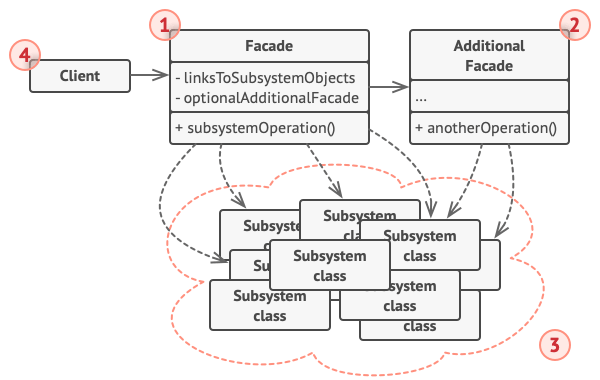
\includegraphics[width=\linewidth]{figs/facade.png}\\
    \item \textbf{Decorator:} provides an enhanced interface to its subject. It relies on recursive composition to organise an open-ended number of objects that change the skin of a principle object. In other words, a decorator is useful for situations where different combinations of toppings/decorations exist for a specific object, i.e. choice of toppings on Pizza, or choice of milk, sugar, water temperature on coffee.\\
    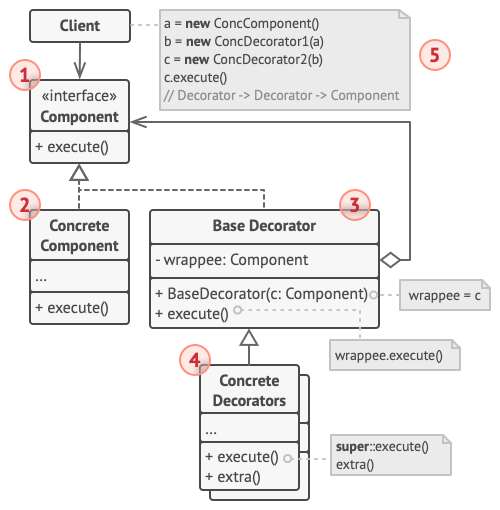
\includegraphics[width=\linewidth]{figs/decorator.png}\\
    \item \textbf{Builder:} is a creational pattern which uses domain knowledge to create a complex object while hiding the internal representation of the object from the client. In other words, builder has a certain algorithm (set of steps) that can be extensible to different implementations of it's steps.\\
    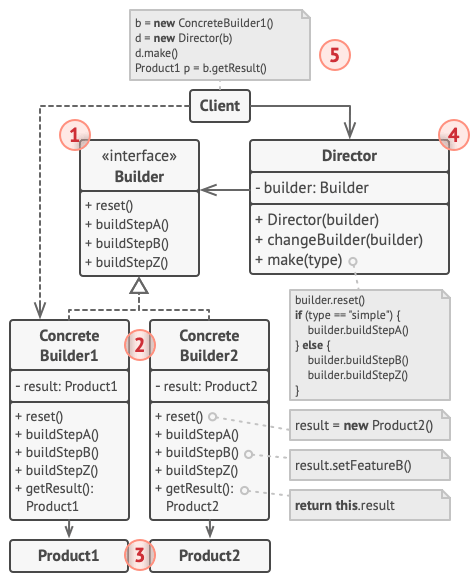
\includegraphics[width=\linewidth]{figs/builder.png}\\
    \item \textbf{Adapter:} resolves incompatible interfaces as well as provide a new stable/intermediate interface to multiple legacy interfaces.\\
    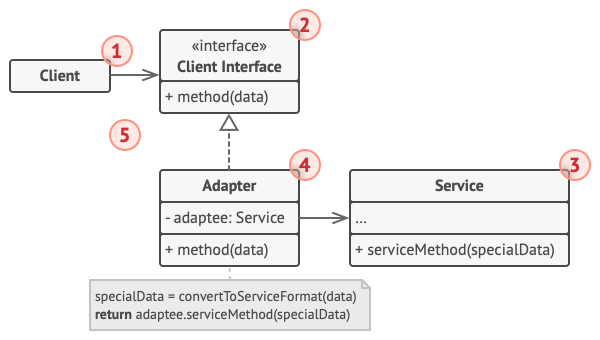
\includegraphics[width=\linewidth]{figs/adapter.png}\\
    \item \textbf{Singleton:} exactly one instance of a Singleton class should exist. Objects need a global and single point of access. So we can define a static method that returns the same instance of the class every time it is called.\\
    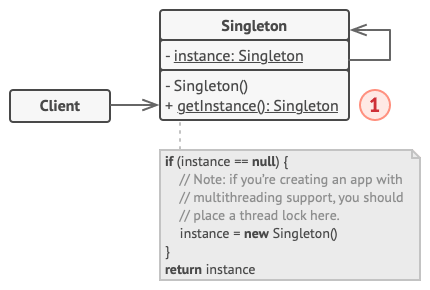
\includegraphics[width=\linewidth]{figs/singleton.png}\\
    \item \textbf{Factory:} Concrete factory is a simplified factory of the GoF abstract factory pattern.\\
    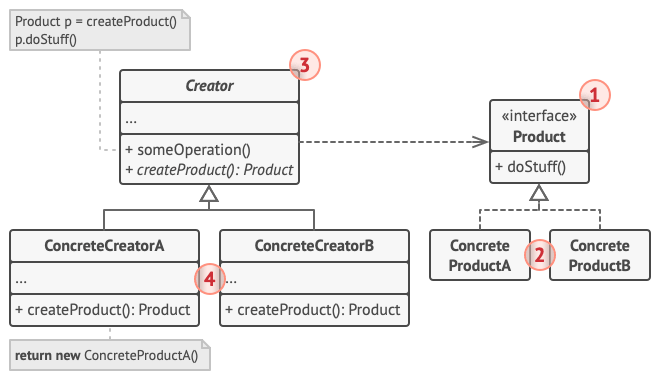
\includegraphics[width=\linewidth]{figs/factory.png}\\
    \item \textbf{Composite:} \textit{Problem} How to treat a group or composite structure of objects the same way (polymorphically) as a non-composite (atomic) object?\\
    \textit{Solution} Define classes for composite and atomic objects so that they implement the same interface.\\
    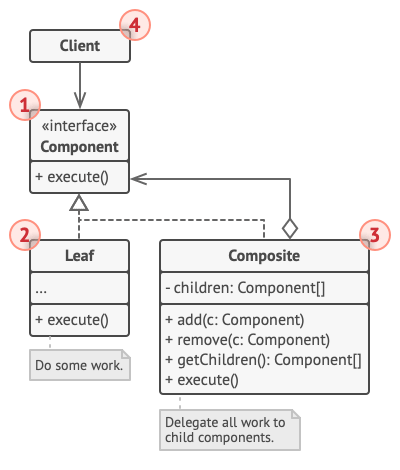
\includegraphics[width=\linewidth]{figs/composite.png}\\
    \item \textbf{Template:} \textit{Problem} How to build generic components that are easy to extend and use without replicating code?
    \textit{Solution} Define a family of algorithms, encapsulate each one, and make them interchangeable. Allows the implementation of invariant parts of an algorithm once and leave it to the subclasses to implement the behaviour that can vary.\\
    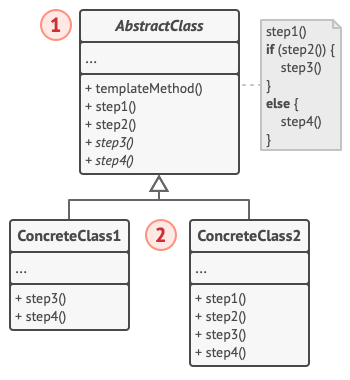
\includegraphics[width=\linewidth]{figs/template.png}\\
    \item \textbf{Strategy:} \textit{Problem} How to design for varying, but related, algorithms or policies?\\
    \textit{Solution} Define each algorithm/policy/strategy in a separate class, with a common interface.\\
    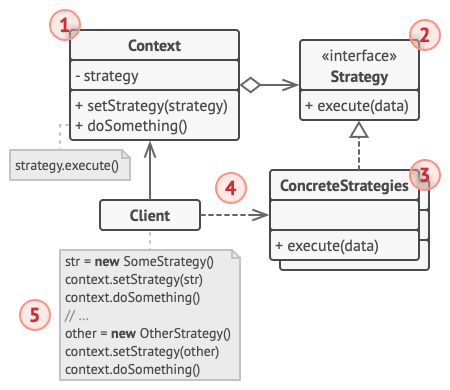
\includegraphics[width=\linewidth]{figs/strategy.png}\\
    \item \textbf{Observer:} \textit{Problem} Different kinds of subscriber objects are interested in the state changes or events of a publisher object, and want to react in their own unique way when the publisher generates an event. Moreover, the publisher wants to maintain low coupling to the subscribers.
    \textit{Solution} Define a "subscriber" or "listener" interface. Subscribers implement this interface. The publisher can dynamically register subscribers who are interested in an event and notify them when an event occurs.\\
    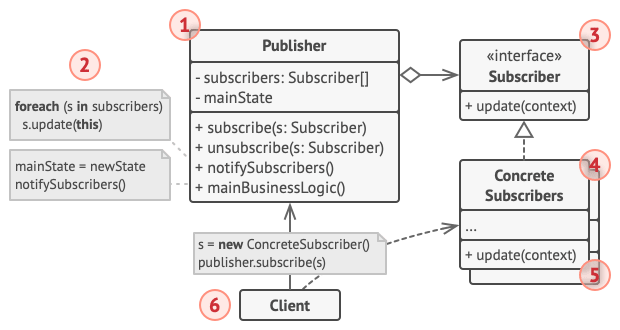
\includegraphics[width=\linewidth]{figs/observer.png}\\
\end{itemize}